%% Supplementary material for the TMC version (tmc.tex). Single self-contained file; references to the main paper are written as numbers.
\documentclass[10pt,journal,compsoc]{IEEEtran}

\usepackage[nocompress]{cite}
\usepackage{amsmath,amssymb,amsfonts}
\let\proof\relax
\let\endproof\relax
\usepackage{amsthm}
\usepackage{algorithm}
\usepackage{algpseudocode}
\usepackage{graphicx}
\usepackage{booktabs}
\usepackage{xcolor}
\usepackage{url}

\newtheorem{assumption}{Assumption}
\newtheorem{definition}{Definition}
\newtheorem{lemma}{Lemma}
\newtheorem{proposition}{Proposition}
\newtheorem{corollary}{Corollary}
\newtheorem{theorem}{Theorem}
\theoremstyle{remark}
\newtheorem{remark}{Remark}
\newtheorem{example}{Example}

\newcommand{\E}{\mathbb{E}}
\newcommand{\Prob}{\mathbb{P}}
\newcommand{\ind}[1]{\mathbf{1}\{#1\}}
\newcommand{\A}{\mathcal{A}}
\newcommand{\I}{\mathcal{I}}
\newcommand{\lab}{\ell}
\newcommand{\Dbar}{\bar{\Delta}}
\newcommand{\ee}{\varepsilon}
\newcommand{\xh}{\hat{x}}

\renewcommand{\thesection}{S\arabic{section}}
\renewcommand{\thetable}{S\arabic{table}}
\renewcommand{\thefigure}{S\arabic{figure}}
\renewcommand{\theremark}{S\arabic{remark}}
\renewcommand{\theexample}{S\arabic{example}}
\begin{document}
\title{Supplementary Material for ``Speak When Sure, Ask When Unsure: Confidence-Aware Status Updates from On-Board Classifiers in Aerial IoT''}
\author{Sameh~Hosny%
\IEEEcompsocitemizethanks{\IEEEcompsocthanksitem S. Hosny is with the Electrical and Computer Engineering Department, American University of Armenia, Yerevan, Armenia.\protect\\
E-mail: sameh.hosny@aua.am}}
\markboth{IEEE Transactions on Mobile Computing}{Hosny: Supplementary Material}
\maketitle

This document supplements the main paper. Equation, section, lemma, proposition, theorem, figure and table numbers without the prefix S refer to the main paper. Section~\ref{sec:smodel} gives the notation and model details, Section~\ref{sec:sexample} a worked example of the belief update and the decision rule, Section~\ref{sec:sproofs} the proofs, and Section~\ref{sec:sresults} additional results.

\section{Notation and Model Details}\label{sec:smodel}
Table~\ref{tab:notation} summarizes the notation. Fig.~\ref{fig:markov} shows the two-state Markov chain of the patch state $X(t)$ in~(1).

\begin{table}[t]
\caption{Main notation}\label{tab:notation}
\centering\footnotesize
\setlength{\tabcolsep}{3pt}
\begin{tabular}{@{}p{0.58\columnwidth}ll@{}}
\toprule
Meaning & Symbol & Defined in\\
\midrule
Patch below the UAV: event or not & $X(t)$ & (1)\\
How often the scene changes & $p_0,p_1$; $\varpi$ & (1), (2)\\
Photo; on-board label, confidence & $Y(t)$; $\lab(t)$, $c(t)$ & (4)\\
Label disagrees with the GS status & $d(t)$ & Sec.~4.4\\
Label from the ground classifier & $\lab^{\rm g}(t)$, $\ee_{\rm g}(c)$ & Assum.~1\\
Silent, send label, send photo & $a(t)\in\{0,1,2\}$ & Sec.~3.4\\
UAV position, blockage & $g(t)$ & (7), (8)\\
Packet decoded & $o(t)$ & (12)\\
Delivery probability; energy & $q_a(g)$; $E_a(g)$ & (9), (10)\\
Energy budget of the mission & $\bar E$ & (11)\\
What the GS status says & $\hat X(t)$ & (12)\\
How long the GS status has been wrong & $\Delta(t)$ (AoII) & (13)\\
What the UAV believes about $\Delta(t)$ & $\pi_t$; $\mu_t$, $S_t$ & (18), (23)\\
Evidence of a frame that the GS is wrong & $\Lambda_t$ & (20)\\
Value of an action; its energy price & $G_a$; $Z(t)$, $V$ & Secs.~5, 6\\
\bottomrule
\end{tabular}
\end{table}

\begin{figure}[t]
\centering
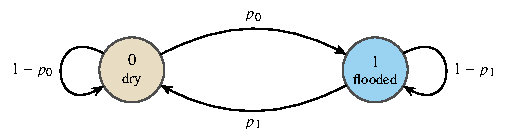
\includegraphics[width=0.55\columnwidth]{figures/fig_markov.pdf}
\caption{Two-state Markov chain of the patch state $X(t)$. A dry patch ($0$) is followed by a flooded one with probability $p_0$, and a flooded patch ($1$) by a dry one with probability $p_1$. With $p_0,p_1<\frac12$ the state tends to persist from one footprint to the next.}
\label{fig:markov}
\end{figure}

\subsection{Classifier Outputs}
Fig.~\ref{fig:inference} shows the classifier outputs that motivate Assumption~1. In (a), the on-board model, its noisiest variant and the ground model are close to calibrated after isotonic calibration, so~(4) holds to a good approximation. In (b), the measured error rate of the on-board label follows $1-c$ across confidence bins, and the error rate of the ground model also falls as the on-board confidence grows, which is why we write $\ee_{\rm g}(c)$. In (c), the errors come in runs over consecutive footprints, which violates Assumption~1(ii) and motivates the tempered update~(21).

\begin{figure*}[t]
\centering
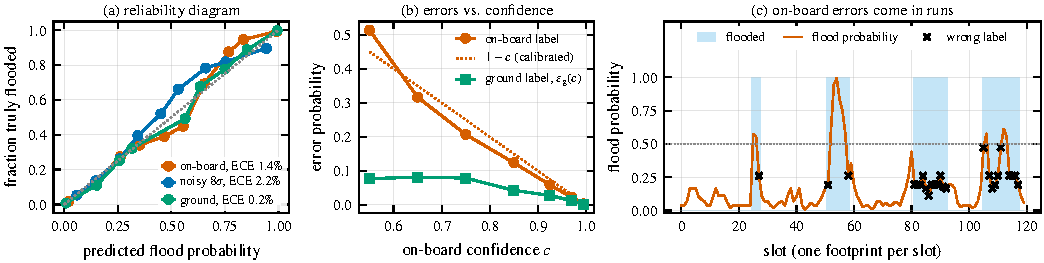
\includegraphics[width=\textwidth]{figures/fig_inference.pdf}
\caption{Classifier outputs on the Sen1Floods11 test chips. (a) Reliability diagram: fraction of truly flooded footprints versus the predicted flood probability, for the on-board model, its noisiest variant and the ground model, with their expected calibration errors (ECE). All three are well calibrated. (b) Error rate of the on-board and ground labels versus the on-board confidence $c$. The on-board error follows $1-c$ (dotted); the ground model also errs more on hard frames. (c) $120$ consecutive footprints of one test chip: flooded footprints shaded, on-board flood probability (line) and wrong labels (crosses). Errors come in runs, mostly missed floods.}
\label{fig:inference}
\end{figure*}

\subsection{An AoII Example}
Table~\ref{tab:aoiiex} gives an example from the flood scenario over eight slots. In slot $2$ a wrong ``flooded'' label is delivered, so the GS becomes wrong in slot $3$ although the scene has not changed. In slot $4$ the patch floods, and the GS happens to become correct. In slot $4$ the UAV also delivers a wrong ``dry'' label, so the GS is wrong again in slots $5$ and $6$, until a correct label sent in slot $6$ fixes it.

\begin{table}[t]
\caption{AoII in a flood example ($1$: flooded, $0$: dry)}\label{tab:aoiiex}
\centering\footnotesize
\setlength{\tabcolsep}{5pt}
\begin{tabular}{@{}lcccccccc@{}}
\toprule
Slot $t$ & 1 & 2 & 3 & 4 & 5 & 6 & 7 & 8\\
\midrule
True state $X(t)$ & 0 & 0 & 0 & 1 & 1 & 1 & 1 & 1\\
Delivered label in slot $t$ & -- & 1 & -- & 0 & -- & 1 & -- & --\\
GS status $\hat X(t)$ & 0 & 0 & 1 & 1 & 0 & 0 & 1 & 1\\
AoII $\Delta(t)$ & 0 & 0 & 1 & 0 & 1 & 2 & 0 & 0\\
\bottomrule
\end{tabular}
\end{table}

\subsection{Undetected Errors and Harvesting}
The main paper assumes that every decoded packet is correct and that the budget is a long-run average. The two remarks below relax these assumptions.

\begin{remark}[Undetected errors]\label{rem:flip}
Suppose instead that a decoded label is flipped with a small probability $\ee_{\rm u}$. Because the label is binary, a flipped disagreeing label equals the current GS status, so it changes nothing. A bit error on the link can therefore cancel an update but cannot make a correct GS status wrong. Its only effect is to replace $q_1(g)$ by $q_1(g)(1-\ee_{\rm u})$ in everything that follows. An undetected error in a raw frame corrupts the photo rather than the label, and its effect can be folded into the ground error $\ee_{\rm g}(c)$.
\end{remark}

\begin{remark}[Harvesting battery]\label{rem:harvest}
If the UAV, or a ground sensor running the same policy, harvests energy into a finite battery with content $B(t)$, the constraint becomes that the battery never runs empty. The perturbed Lyapunov method of~\cite{huang2013eh} applies the same derivation to the battery, shifted by a constant $\theta$, and yields~(30) with $\lambda(t)=\theta-B(t)$: energy becomes expensive when the battery is low. With a battery capacity of at most $\theta$, the price stays nonnegative, so Proposition~1 still applies. By the argument behind Theorem~1, choosing $\theta\ge E_{\max}+V(\Delta_{\max}+1)/E_{\min}$ ensures that the UAV never chooses an action that the battery cannot pay for.
\end{remark}

\section{Worked Example}\label{sec:sexample}
This example follows one UAV over two slots, first through the belief update of Section~4.4 and then through the decision rule~(30). The numbers are illustrative and are taken from the evaluation setting of Section~7.

\begin{example}\label{ex:belief}
Let the GS report ``not flooded'' ($\hat X(t)=0$), and let the UAV hold the belief $\pi^-_t(0)=0.95$, $\pi^-_t(1)=0.05$: it is fairly sure the GS is right. A frame then arrives with label ``flooded'' and confidence $c=0.9$, so $d(t)=1$. With $\varpi_0=0.81$ and $\varpi_1=0.19$,~(20) gives $\Lambda_t=(0.81/0.19)(0.9/0.1)=38.4$: the frame is $38$ times more likely if the GS is wrong. With exact Bayes' rule ($\nu=1$),~(21) gives $\mu_t=0.05\cdot38.4/(0.95+0.05\cdot38.4)=0.67$: one confident frame makes the GS more likely wrong than right. With $\nu=0.5$ the same frame gives only $\mu_t=0.25$, and with $\nu=0.25$ it gives $\mu_t=0.12$. Suppose the UAV stays silent. The prediction~(22) with $p_0=0.039$ and $p_1=0.166$ gives $\mu^-_{t+1}=0.23$ for $\nu=0.5$. If the next frame again says ``flooded'' with $c=0.9$, the belief rises to $\mu_{t+1}=0.65$. With the tempered update, the UAV therefore needs two consistent frames to become as convinced as one frame makes it under exact Bayes' rule. The next two parts of the example show what the UAV does in each of these two slots.
\end{example}

\subsection{Gains of the Three Actions}
\setcounter{example}{0}
\begin{example}[continued]
In slot $t$ of Example~\ref{ex:belief} with $\nu=0.5$, the belief is $\mu_t=0.25$ and $S_t=0.49$, and the ground error at $c=0.9$ is $\ee_{\rm g}=0.028$ (Fig.~\ref{fig:inference}(b)). With $\xh=0$, $r=p_0=0.039$ and $w=p_1=0.166$. Lemma~2 gives $G_1=-0.37$ and $G_2=0.30$: sending the label would more likely harm than help, while asking the ground would help. In slot $t+1$, after the second disagreeing frame, $\mu_{t+1}=0.65$ and the gains become $G_1=0.94$ and $G_2=1.21$. Now the GS is probably wrong, and the label is worth sending.
\end{example}

\subsection{Decision}
\setcounter{example}{0}
\begin{example}[continued]
Let the UAV be $1.2$\,km from the GS, where $q_1\approx1$, $q_2=0.78$, $E_1=20$\,mJ and $E_2=190$\,mJ. In slot $t$, the label has $q_1G_1<0$, and the upload has $q_2G_2=0.23$, so~(30) uploads the frame if $\lambda/V<0.23/0.19=1.2$\,J$^{-1}$ and stays silent otherwise. In slot $t+1$, $q_1G_1=0.94$ and $q_2G_2=0.95$ are almost equal, but the label costs a tenth of the upload, so the UAV sends the label for any price between about $0.05$ and $47$\,J$^{-1}$. At the price $\lambda/V=2$\,J$^{-1}$ used in Fig.~2, the UAV thus waits in slot $t$ and sends the label in slot $t+1$.
\end{example}

\section{Proofs}\label{sec:sproofs}
\subsection{Proof of Lemma~3}\label{app:mono}
Let $y=\Lambda_t^{\nu}$, which increases with $\Lambda_t$. By~(21), the mass at every $\delta>0$ is multiplied by $y/D$ and the mass at $\delta=0$ by $1/D$, with $D=1-\mu^-_t+\mu^-_ty$. Hence
\[
S_t=\frac{y\,S^-_t}{D},\qquad 1-\mu_t=\frac{1-\mu^-_t}{D},
\]
and $AS_t-B(1-\mu_t)=N/D$ with $N=AyS^-_t-B(1-\mu^-_t)$. Both $N$ and $D$ are affine in $y$, so the derivative of $N/D$ with respect to $y$ has the sign of
\begin{multline*}
AS^-_t\big(1-\mu^-_t+\mu^-_ty\big)-\big(AyS^-_t-B(1-\mu^-_t)\big)\mu^-_t\\
=(1-\mu^-_t)\big(AS^-_t+B\mu^-_t\big)\ \ge\ 0.
\end{multline*}
Since $D>0$, $N/D$ is nondecreasing in $y$, and hence in $\Lambda_t$. \hfill$\blacksquare$

\subsection{Proof of Proposition~2}\label{app:threshold}
Let $f_a=Vq_aG_a-\lambda E_a$ be the objective of~(30), so $f_0=0$. Since $r,w<\frac12$ and $\ee_{\rm g}\le1$, both gains have the form $AS_t-B(1-\mu_t)$ with $A,B\ge0$: for $G_2$, $A=(1-\ee_{\rm g})(1-2w)$ and $B=\ee_{\rm g}(1-2r)$, and for $G_1$ with $d(t)=1$, $A=1-2w$ and $B=1-2r$. The difference $q_1G_1-q_2G_2$ has the same form, with
\[
A=(1-2w)\big(q_1-q_2(1-\ee_{\rm g})\big),\qquad B=(1-2r)\big(q_1-q_2\ee_{\rm g}\big),
\]
both nonnegative because $q_2\le q_1$. By Lemma~3, $f_2-f_0=Vq_2G_2-\lambda E_2$ and $f_1-f_2=V(q_1G_1-q_2G_2)-\lambda(E_1-E_2)$ are nondecreasing in $\Lambda_t$, and so is their sum $f_1-f_0$.

(a) If $d(t)=1$, then $\Lambda_t$ increases in $c$. Order the actions as $0\prec2\prec1$. The differences between consecutive actions in this order are nondecreasing in $c$, so $f_a$ has increasing differences in $(a,c)$. By Topkis' theorem, the set of maximizers of $f_a$ is nondecreasing in $c$ in the strong set order, so its smallest and largest elements are both nondecreasing in $c$. Algorithm~1 selects the smallest maximizer, breaking ties toward silence and then toward the raw upload. Hence the action moves from 0 to 2 to 1 as $c$ grows, which defines $c_{\rm r}\le c_{\lab}$.

(b) If $d(t)=0$, then $G_1=0$ by Proposition~1, so $f_1=-\lambda E_1\le f_0$ and the label is never strictly preferred to silence. Now $\Lambda_t$ decreases in $c$, so $f_2-f_0$ is nonincreasing in $c$, and the set of $c$ for which $f_2>f_0$ is an interval of the form $\{c\le c^0_{\rm r}\}$.

(c) For fixed $\mu^-_t$ and $\Lambda_t$, $S^-_t$ appears in $N/D$ only in the numerator, with coefficient $Ay\ge0$. So $f_a-f_0$ is nondecreasing in $S^-_t$ for $a\in\{1,2\}$, and a slot in which some action beats silence still has one when $S^-_t$ grows. Each $f_a-f_0$ with $a\neq0$ decreases in $\lambda$, so a slot in which silence is optimal remains so when $\lambda$ grows. \hfill$\blacksquare$

\subsection{Proof of Theorem~1}\label{app:budget}
We first bound the gains. Since the belief is truncated at $\Delta_{\max}$, $S_t=\E_{\pi_t}[(\Delta+1)\ind{\Delta>0}]\le\Delta_{\max}+1$. By~(28) and~(29), $G_a\le S_t$ for $a\in\{1,2\}$, because the negative terms can be dropped and $(1-2w)(1-\ee_{\rm g})\le1$. With $q_a\le1$, $Vq_aG_a\le V(\Delta_{\max}+1)$.

Let $z^\star=V(\Delta_{\max}+1)/E_{\min}$. If $Z(t)>z^\star$, then for $a\in\{1,2\}$,
\[
Vq_aG_a-Z(t)E_a(g)<V(\Delta_{\max}+1)-z^\star E_{\min}=0=f_0,
\]
so CA-DPP stays silent, and~(31) gives $Z(t+1)=\max\{Z(t)-\bar E,0\}\le Z(t)$. If $Z(t)\le z^\star$, then $Z(t+1)\le Z(t)+E_{\max}\le z^\star+E_{\max}$. Starting from $Z(0)=0$, induction on $t$ gives $Z(t)\le z^\star+E_{\max}=Z_{\max}$ for all $t$. Inserting this bound in~(32) gives the energy bound for every $T$, and taking expectations and $T\to\infty$ gives~(11). \hfill$\blacksquare$


\section{Additional Results}\label{sec:sresults}
This section gives the details of the checks summarized in Section~7.9.

\subsection{Sample Path}
\begin{figure}[!tb]
\centering
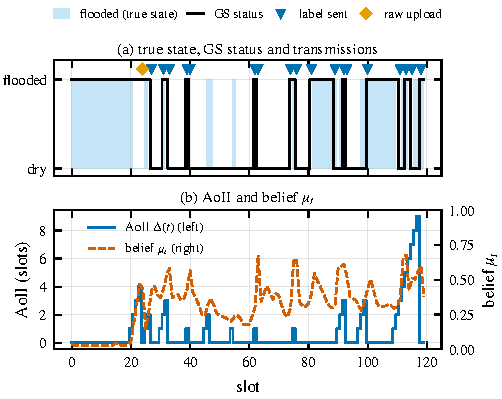
\includegraphics[width=0.8\columnwidth]{figures/fig_path.pdf}
\caption{Sample path of CA-DPP over $120$ slots at $\bar E=0.5$\,mJ/slot ($V=0.01$, $\nu=0.25$). (a) True state (shaded when flooded), GS status, and the slots in which the UAV sends a label (triangles) or uploads the frame (diamond). (b) AoII of the GS status (left axis) and the belief $\mu_t$ that the GS is wrong (right axis). The belief rises with each disagreeing frame until a label is sent, which resets the AoII.}
\label{fig:path}
\end{figure}

Fig.~\ref{fig:path} shows how CA-DPP works. The AoII spike at the end shows the cost of waiting: the tempered update discounts the first disagreeing frames, so the belief rises more slowly than the true error.

\subsection{The Weight $V$ and the Role of Mobility}\label{res:V}
\begin{figure}[!tb]
\centering
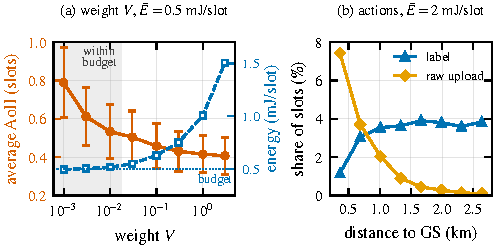
\includegraphics[width=0.8\columnwidth]{figures/fig_V_mix.pdf}
\caption{(a) Average AoII of CA-DPP (left axis) and energy spent (right axis, dashed) versus $V$ at $\bar E=0.5$\,mJ/slot. In the shaded range the energy stays within $4\%$ of the budget (dotted); a larger $V$ lowers the AoII but overspends. (b) Share of unblocked slots with a label or a raw upload versus the distance to the GS, at $\bar E=2$\,mJ/slot. Uploads dominate near the GS; labels take over beyond about $0.8$\,km.}
\label{fig:Vmix}
\end{figure}

Fig.~\ref{fig:Vmix}(a) shows the trade-off governed by $V$ at $0.5$\,mJ/slot. Raising $V$ from $10^{-3}$ to $3$ lowers the AoII from $0.79$ to $0.41$. A larger $V$, however, lets the debt grow before it raises the price: over about $27{,}000$ slots the energy spent rises from $0.50$ to $1.51$\,mJ/slot. Values of $V$ up to $10^{-2}$ stay within $4\%$ of the budget. Theorem~1 holds for every $V$, but the transient excess grows with $V$, so $V$ must match the mission length.

Fig.~\ref{fig:Vmix}(b) shows how CA-DPP exploits the trajectory. Within $850$\,m of the GS, where uploads are cheap and reliable, it uploads the frame in $5.9\%$ of the unblocked slots and sends labels in $2.0\%$. Beyond $2.15$\,km it uploads in only $0.1\%$ and sends labels in $3.8\%$. The UAV asks the ground when asking is cheap, although the distance enters~(30) only through $q_a(g)$ and $E_a(g)$.

\subsection{Distance to the Optimal Policy}\label{res:opt}
Section~6 leaves the gap between CA-DPP and the optimal policy of (P) open, and computing that optimum is out of reach, since the belief has $\Delta_{\max}+1$ entries. A lower bound on it can be computed, however. A controller that also observes $X(t)$, and therefore the AoII and whether the on-board label is right, can imitate any policy of (P), so the optimal AoII of this full-information controller under the same budget is a lower bound on the optimum of (P). Its problem is a constrained Markov decision process over $X(t)$, the AoII, the orbit position and the blockage state. We solve its Lagrangian relaxation by value iteration for a range of energy prices, with the AoII capped (which can only lower the bound), and obtain the bound at each energy level by weak duality. To compare against the bound without confounding factors, we use a synthetic model that satisfies Assumption~1: $X(t)$ follows the Markov chain fitted to the data, and in each slot the outputs of the two classifiers are drawn jointly from data slots with the same state, so the errors are independent over time. CA-DPP then uses $\nu=1$. CA-DPP and the AoII-threshold policy are tuned as in Section~7.5 and run six times for $10^5$ slots.

\begin{table}[t]
\caption{Synthetic model with independent errors: average AoII of CA-DPP and of the AoII-threshold policy (mean of six runs), and the lower bound at the energy each policy spends. The gap is the excess over the bound; the true gap to the optimal policy is smaller.}\label{tab:optgap}
\centering\footnotesize
\begin{tabular}{@{}ccccccc@{}}
\toprule
 & \multicolumn{3}{c}{CA-DPP} & \multicolumn{3}{c}{AoII threshold}\\
\cmidrule(lr){2-4}\cmidrule(l){5-7}
$\bar E$ (mJ/slot) & AoII & bound & gap & AoII & bound & gap\\
\midrule
$0.25$ & $0.878$ & $0.701$ & $+25\%$ & $1.208$ & $0.706$ & $+71\%$\\
$0.5$ & $0.624$ & $0.497$ & $+25\%$ & $0.941$ & $0.686$ & $+37\%$\\
$1$ & $0.389$ & $0.320$ & $+22\%$ & $0.464$ & $0.335$ & $+38\%$\\
$2$ & $0.348$ & $0.306$ & $+14\%$ & $0.464$ & $0.335$ & $+38\%$\\
\bottomrule
\end{tabular}
\end{table}

Table~\ref{tab:optgap} shows that CA-DPP is within $14\%$ to $25\%$ of the bound at every budget, and the gap shrinks as energy grows. The bound credits the controller with knowing $X(t)$, which no policy of (P) can match, so CA-DPP is at least this close to the optimal policy. The AoII-threshold policy is $37\%$ to $71\%$ above the bound; at the larger budgets it spends less than allowed, because even with $k=1$ it sends only labels that disagree with the GS. In this model CA-DPP also stays ahead of the threshold policy at $2$\,mJ/slot, by $25\%$ in AoII, while on the real traces the two tie at this budget (Section~7.6). The difference between the two settings is the correlation of the errors, which Section~\ref{res:corr} examines.

\subsection{Correlated Errors}\label{res:corr}
On the real traces the on-board errors come in runs (Section~7.2). To isolate their effect, we extend the synthetic model with an error indicator that follows a two-state Markov chain with the measured error rate $8.2\%$ and persistence $\Prob\{\text{wrong at }t+1\mid\text{wrong at }t\}=\varrho$. Given the state and the indicator, the confidence and the ground output are drawn from data slots with the same state and the same correctness, so the classifier stays calibrated. We vary $\varrho$ from $0.082$ (independent errors) to $0.8$; the real traces have $\varrho=0.56$. CA-DPP runs with the rule of Section~4.4 and, for comparison, with $\nu=1$.

\begin{table}[t]
\caption{Synthetic model with correlated errors: AoII reduction of CA-DPP relative to the AoII-threshold policy (mean of six paired runs; negative favors CA-DPP), with $\nu$ from the rule and with $\nu=1$.}\label{tab:corr}
\centering\footnotesize
\begin{tabular}{@{}cccccc@{}}
\toprule
 & & \multicolumn{2}{c}{$\bar E=0.5$\,mJ/slot} & \multicolumn{2}{c}{$\bar E=2$\,mJ/slot}\\
\cmidrule(lr){3-4}\cmidrule(l){5-6}
$\varrho$ & rule $\nu$ & rule $\nu$ & $\nu=1$ & rule $\nu$ & $\nu=1$\\
\midrule
$0.082$ & $1.00$ & $-23\%$ & $-23\%$ & $-23\%$ & $-23\%$\\
$0.3$ & $0.62$ & $-21\%$ & $-21\%$ & $-7\%$ & $-6\%$\\
$0.56$ & $0.32$ & $-20\%$ & $-17\%$ & $-4\%$ & $-1\%$\\
$0.8$ & $0.12$ & $-34\%$ & $-13\%$ & $-10\%$ & $-1\%$\\
\bottomrule
\end{tabular}
\end{table}

Table~\ref{tab:corr} shows two effects. With independent errors, CA-DPP lowers the AoII of the threshold policy by about $23\%$ at both budgets. As the errors become more persistent, the advantage at $2$\,mJ/slot shrinks, because a run of wrong labels looks like strong evidence to a belief that counts each frame separately; with $\nu=1$ it disappears. The rule for $\nu$ recovers part of it, and at $0.5$\,mJ/slot it keeps CA-DPP ahead at every persistence. This suggests that the tie on the real traces at large budgets comes from the correlated errors, which the belief does not model, and a belief that models the error process is the next step (Section~8).

\subsection{Robustness Checks}\label{res:robust}
\emph{Choice of $\nu$.} The main results select $\nu$ on the tuning folds. Table~\ref{tab:nu} repeats the trace-driven evaluation with $\nu$ set instead by the correlation rule of Section~4.4, which gives $\nu$ between $0.31$ and $0.35$ for the base model and between $0.30$ and $0.42$ for the noisy variants; everything else, including the folds and the random numbers, is unchanged. With the rule, CA-DPP lowers the AoII of the threshold policy by $16\%$ (paired relative change) at $0.5$\,mJ/slot (paired $p=0.003$) and by $11\%$ and $15\%$ at $5$ and $10$\,mJ/slot ($p=0.015$ and $p=0.008$ on the five fold means), where the tuned version ties. At $0.25$\,mJ/slot, however, its AoII rises from $0.65$ to $0.87$ and it only ties with the threshold policy, and with the weakest classifier its AoII rises from $0.64$ to $0.78$, still $41\%$ below the threshold policy. The best discount therefore depends on the budget, and choosing it per budget on tuning data, as in the main results, is the safer default. Repeating the rule run with ten folds gives the same picture: a tie at $0.25$\,mJ/slot and reductions of $7\%$ at $0.5$\,mJ/slot and of $31\%$ and $40\%$ with the two weakest classifiers.

\begin{table}[t]
\caption{Average AoII of CA-DPP with $\nu$ selected on the tuning folds (main results) and with $\nu$ from the correlation rule, and of the AoII-threshold policy (mean of $20$ held-out runs, $5$-fold cross-validation). The last two rows use the two weakest on-board classifiers at $\bar E=0.5$\,mJ/slot.}\label{tab:nu}
\centering\footnotesize
\begin{tabular}{@{}lccc@{}}
\toprule
 & \multicolumn{2}{c}{CA-DPP} & AoII\\
\cmidrule(lr){2-3}
Setting & tuned $\nu$ & rule $\nu$ & threshold\\
\midrule
$\bar E=0.25$\,mJ/slot & $0.645$ & $0.867$ & $0.925$\\
$\bar E=0.5$\,mJ/slot & $0.526$ & $0.479$ & $0.564$\\
$\bar E=1$\,mJ/slot & $0.418$ & $0.356$ & $0.363$\\
$\bar E=2$\,mJ/slot & $0.390$ & $0.337$ & $0.352$\\
$\bar E=5$\,mJ/slot & $0.360$ & $0.309$ & $0.352$\\
$\bar E=10$\,mJ/slot & $0.341$ & $0.291$ & $0.352$\\
accuracy $83.9\%$ & $0.581$ & $0.570$ & $0.809$\\
accuracy $81.8\%$ & $0.643$ & $0.775$ & $1.312$\\
\bottomrule
\end{tabular}
\end{table}

The selection itself is noisy. With $\nu$ fixed and only $V$ tuned, CA-DPP reaches an AoII of $0.41$, $0.44$, $0.47$, $0.55$ and $0.72$ at $0.5$\,mJ/slot for $\nu=0.14$, $0.25$, $0.32$, $0.5$ and $1$, and $0.34$, $0.34$, $0.34$, $0.36$ and $0.41$ at $2$\,mJ/slot. Exact Bayes' rule ($\nu=1$) is clearly the worst, which confirms that the tempering matters, and several fixed values do better than the tuned version in Table~3, because the selection on four folds sometimes picks a poor value. The main results are therefore conservative.

\emph{Exact energy.} The energy model~(10) replaces the fading average by its value at the mean SNR. We repeated the budget and accuracy sweeps with the exact average over the fading, computed by numerical integration, and retuned every policy. The AoII of CA-DPP changes by at most $4.2\%$ across budgets and $6.7\%$ across classifiers, its relative change against the threshold policy moves by at most $6$ percentage points, and no significant comparison changes sign.

\emph{A belief-threshold baseline.} Once the belief is available, a simpler policy may seem enough. We therefore tested a rule that sends the label whenever the belief $\mu_t$ that the GS is wrong exceeds a threshold. It uses the same belief as CA-DPP with $\nu=0.25$, never uploads raw frames, and has its threshold chosen per budget on the tuning folds. At $0.25$, $0.5$, $1$, $2$, $5$ and $10$\,mJ/slot its average AoII is $0.75$, $0.47$, $0.37$, $0.37$, $0.37$ and $0.37$, against $0.65$, $0.53$, $0.42$, $0.39$, $0.36$ and $0.34$ for CA-DPP, and none of these differences is significant (paired $p\ge0.10$). The belief is therefore the part of CA-DPP that carries most of its gain over the AoII-threshold policy. What the controller adds is control of the energy. The threshold rule meets a budget only through tuning on past data, with no guarantee, and its energy use stops near $0.65$\,mJ/slot because it never uploads; CA-DPP tracks the budget through the queue with the guarantee of Theorem~1 and adapts its thresholds to the link and the energy price in every slot (Proposition~2).

\emph{Statistics.} Runs on the same fold share chips, so the $20$ held-out runs are not fully independent. Tested on the five fold means instead, the reductions with the two weakest classifiers remain significant ($p=0.035$ and $p=0.014$, all five folds), whereas the $0.25$\,mJ/slot reduction, seen in four of five folds, has $p=0.17$. The large gains over the pre-identification and age-threshold policies hold in every fold up to $5$\,mJ/slot and in four of five folds at $10$\,mJ/slot.

% Generated by IEEEtran.bst, version: 1.14 (2015/08/26)
\begin{thebibliography}{1}
\providecommand{\url}[1]{#1}
\csname url@samestyle\endcsname
\providecommand{\newblock}{\relax}
\providecommand{\bibinfo}[2]{#2}
\providecommand{\BIBentrySTDinterwordspacing}{\spaceskip=0pt\relax}
\providecommand{\BIBentryALTinterwordstretchfactor}{4}
\providecommand{\BIBentryALTinterwordspacing}{\spaceskip=\fontdimen2\font plus
\BIBentryALTinterwordstretchfactor\fontdimen3\font minus
  \fontdimen4\font\relax}
\providecommand{\BIBforeignlanguage}[2]{{%
\expandafter\ifx\csname l@#1\endcsname\relax
\typeout{** WARNING: IEEEtran.bst: No hyphenation pattern has been}%
\typeout{** loaded for the language `#1'. Using the pattern for}%
\typeout{** the default language instead.}%
\else
\language=\csname l@#1\endcsname
\fi
#2}}
\providecommand{\BIBdecl}{\relax}
\BIBdecl

\bibitem{huang2013eh}
L.~Huang and M.~J. Neely, ``Utility optimal scheduling in energy-harvesting
  networks,'' \emph{IEEE/ACM Trans. Netw.}, vol.~21, no.~4, pp. 1117--1130,
  2013.

\end{thebibliography}
\end{document}
